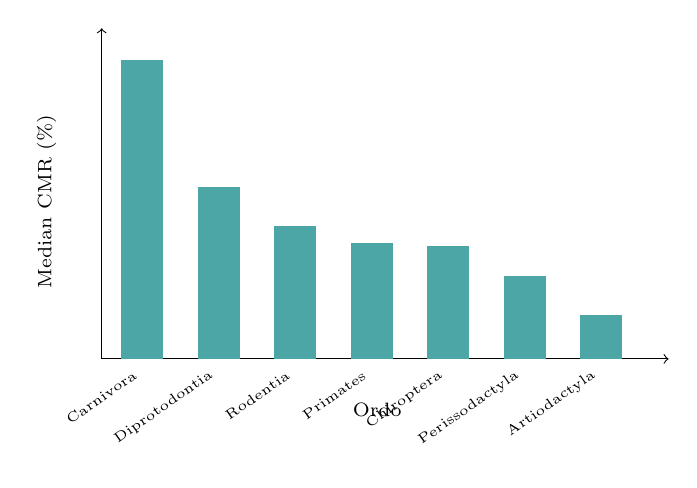
\begin{tikzpicture}[x=1cm,y=1cm]
\draw[->] (0,0) -- (7.2,0);
\draw[->] (0,0) -- (0,4.2);
\node[font=\scriptsize] at (3.5,-0.65) {Ordo};
\node[font=\scriptsize,rotate=90] at (-0.7,2) {Median CMR (\%)};
\fill[teal!70] (0.250,0) rectangle (0.784,3.800);
\node[font=\tiny,rotate=35,anchor=east] at (0.522,-0.12) {Carnivora};
\fill[teal!70] (1.221,0) rectangle (1.756,2.185);
\node[font=\tiny,rotate=35,anchor=east] at (1.493,-0.12) {Diprotodontia};
\fill[teal!70] (2.193,0) rectangle (2.727,1.687);
\node[font=\tiny,rotate=35,anchor=east] at (2.465,-0.12) {Rodentia};
\fill[teal!70] (3.164,0) rectangle (3.699,1.473);
\node[font=\tiny,rotate=35,anchor=east] at (3.436,-0.12) {Primates};
\fill[teal!70] (4.136,0) rectangle (4.670,1.435);
\node[font=\tiny,rotate=35,anchor=east] at (4.408,-0.12) {Chiroptera};
\fill[teal!70] (5.107,0) rectangle (5.641,1.049);
\node[font=\tiny,rotate=35,anchor=east] at (5.379,-0.12) {Perissodactyla};
\fill[teal!70] (6.079,0) rectangle (6.613,0.562);
\node[font=\tiny,rotate=35,anchor=east] at (6.351,-0.12) {Artiodactyla};
\end{tikzpicture}